\section{Bayesian Games}

\subsection{First Definition}
A set of games that differ only in their payoffs, a common prior defined over them, and a partition structure over the game for each agent.\\

\textbf{Formally speaking:}

A \textit{Bayesian game} is a tuple $(N, G, P, I)$ where
\begin{itemize}
\item $N$ is a set of agents
\item $G$ is a set of games with $N$ agents each such that if $g, g' \in G$ then for each agent $i \in N$ the strategy space in $g$ is identical to the strategy space in $g'$
\item $P \in \prod(G)$ is a common prior over games, where $\prod(G) $ is the set of all probability distributions over $G$
\item $I = (I_1, \dots , I_N) $ is a set of partitions of $G$, one for each agent
\end{itemize}

Example:\\
 \begin{center}
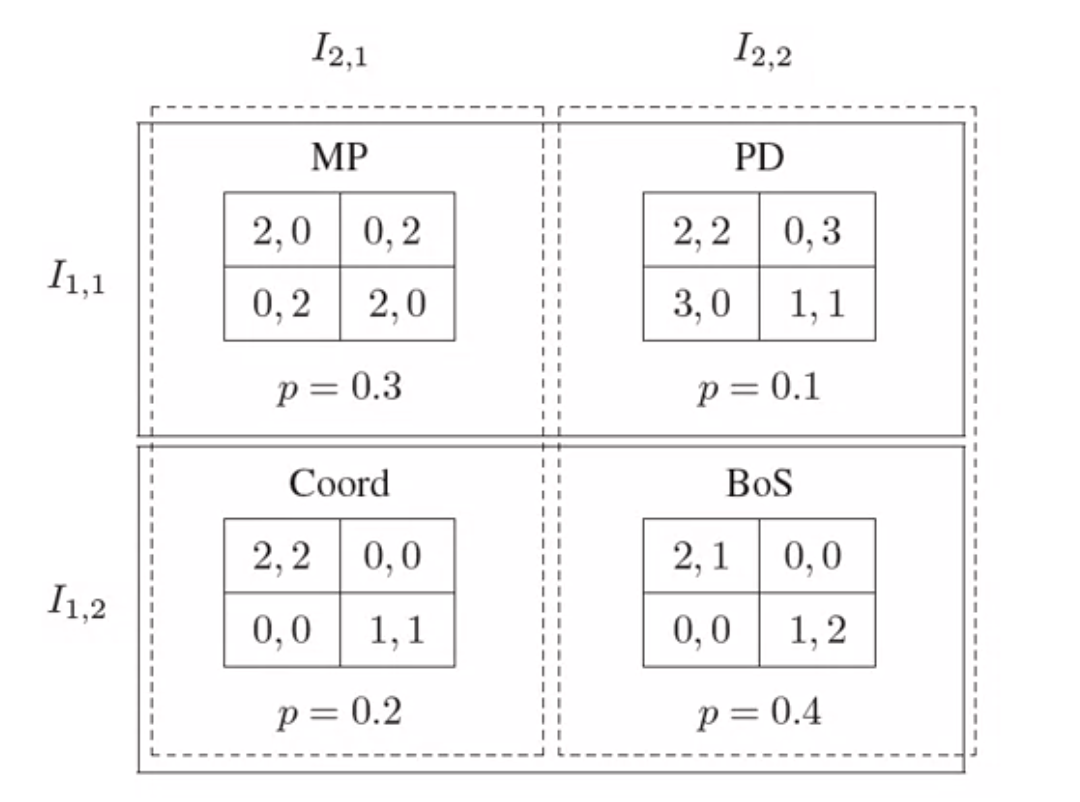
\includegraphics[scale=0.4]{bayesian}\\
\begin{flushleft}
Key:\\
MP - Matching Pennies\\
PD - Prisoners' Dilemma\\
Coord - Coordination Game\\
BoS - Battle of the Sexes
\end{flushleft}
\end{center}
It is going to be randomly decided which game is to be played by the probability factor provided for each game.\\
Here, player 1 won't be able to distinguish between the two games in the first row as well as the two games in the second row. Similar case stands for player 2 with respect to the columns. What this means is that when the players are deciding what action to take, they're going to have to play an action without fully knowing what game is going to be played. And they're going to have to reason about what their opponent is doing without fully knowing what the opponent is going to think. They know the common prior, they know their own equivalence classes and they also know their opponent's equivalence classes.

\subsection{Second Definition}

Directly represent uncertainty over utility function using the notion of \textbf{epistemic types}.\\
Definition:\\
 A  \textit{Bayesian game} is a tuple $(N, A, \Theta, p, u)$ where
\begin{itemize}
\item $N$ is a set of agents
\item $A = (A_1, \dots, A_n)$, where $A_i$ is a set of actions available to player $i$
\item $\Theta = (\Theta_1, \dots , \Theta_n)$ where $\Theta_i$ is the type space of player $i$
\item $p: \Theta \to [0,1] $ is the common prior over types
\item $u = (u_1, \dots, u_n)$,  where $u_i: A \times \Theta \to \mathbb{R}$ is the utility function for player $i$
\end{itemize}
 \begin{center}
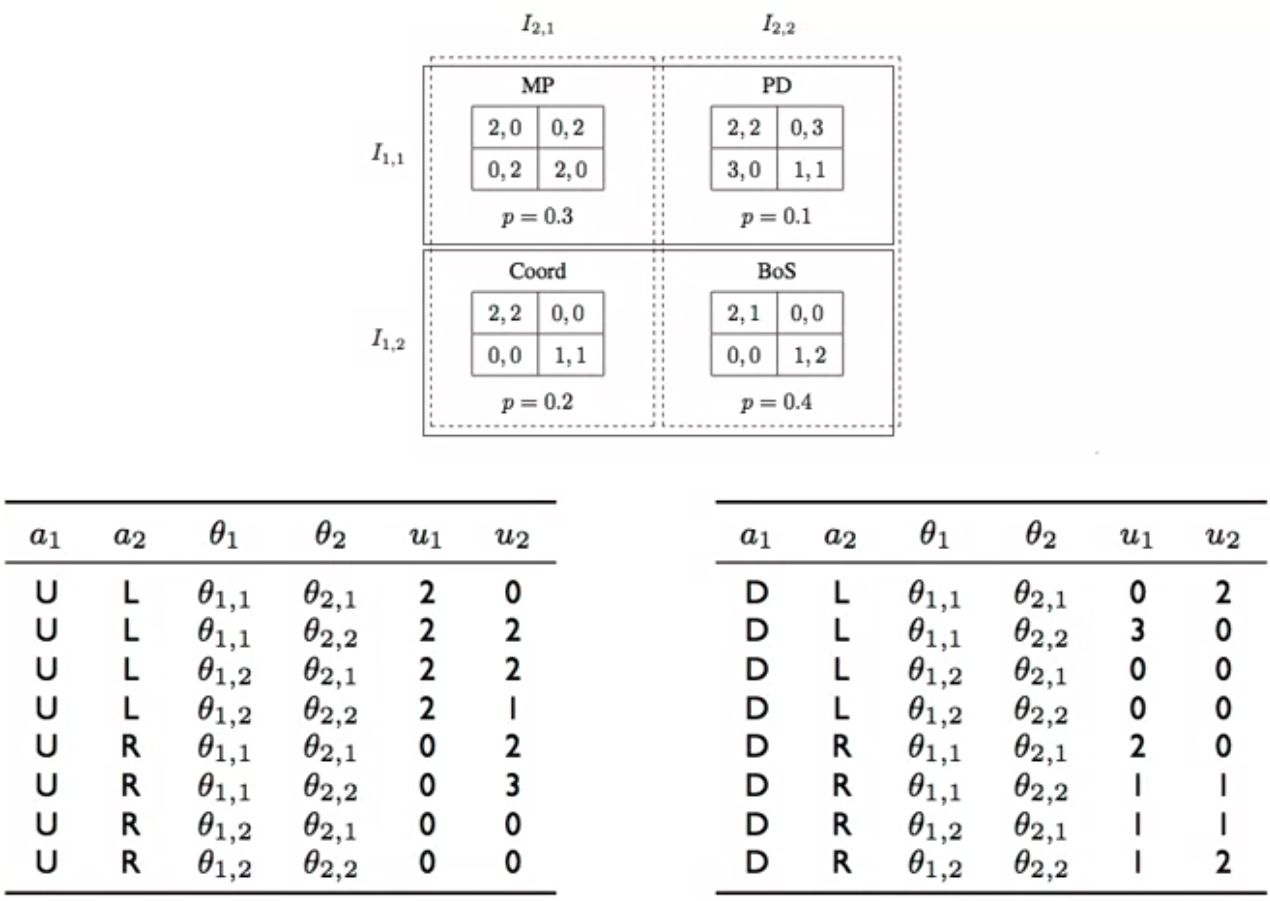
\includegraphics[scale=0.4]{bayesian2}\\
In this figure all the possible moves have been listed out for player 1 and 2, with their corresponding utilities
\end{center}

\subsection{Analyzing Bayesian games}
\subsubsection{Strategies}
Given a Bayesian game $(N, A, \Theta, p, u)$ with finite set of players, actions and types, strategies are defined as follows:
\begin{itemize}
\item \textbf{Pure strategy}: $s_i: \Theta_i \to A_i$
	\begin{itemize}
	\item a choice of a pure action of player $i$ as a function of his or her type
	\end{itemize}
\item \textbf{Mixed strategy}: $s_i: \Theta_i \to \prod(A_i)$
	\begin{itemize}
	\item a choice of a mixed action of player $i$ as a function of his or her type
	\end{itemize}
\end{itemize}
\subsubsection{Expected Utility}
Three standard notions of expected utility are defined.
\begin{itemize}
\item \textit{ex-ante}: The agent knows nothing about anyone's actual type
\item \textit{interim}: an agent knows her own type but not the types of the other agents
\item \textit{ex-post}: the agent knows all agents' types
\end{itemize}
\textbf{Interim Expected Utility}:\\
\begin{itemize}
\item Given a Bayesian game $(N, A, \Theta, p, u)$ with finite set of players, actions and types, $i$'s \textit{interim expected utility} with respect to type $\theta_i$ and a mixed strategy profile $s$ is $$EU_i(s|\theta_i) = \sum_{\theta_{-i} \in \Theta_{-i}}p(\theta_{-i}| \theta_i) \sum_{a \in A}(\prod_{j\in N}s_j(a_j|\theta_j))u_i(a, \theta_i, \theta_{-i})$$
\item $i$'s \textit{ex ante expected utility} with respect to a mixed strategy profile $s$ is $$EU_i(s) = \sum_{\theta_i \in \Theta_I}p(\theta_i)EU_i(s|\theta_i)$$
\end{itemize}
\subsubsection{Bayesian (Nash) Equilibrium}
A Bayesian equilibrium is a mized strategy profile $s$ that satisfies $$s_i \in argmax_{s'_i}EU_i(s'_i,s_{-i}|\theta_i)$$ for each $i$ and $\theta_i \in \Theta_i$\\
If $p(\theta_i)>0$ for all $\theta_i \in \Theta_I$, then this is equivalent to requiring that $$s_i \in argmax_{s'_i}EU_i(s'_i,s_{-i}|\theta_i) = argmax_{s'_i} \sum_{\theta_i}EU_i(s'_i, s_{-i}|\theta_i)$$ for each $i$
\subsection{A Sheriff's Dilemma (Example)}
A sheriff faces an armed suspect and they must simultaneously decide whether to shoot or not :
\begin{itemize}
\item the suspect is a criminal with probability $p$
\item the sheriff would rather shoot if the suspect shoots, but not if the suspect does not
\item the criminal would rather shoot even if the sheriff does not , as the criminal would be caught if does no shooting
\item the innocent suspect would  rather not shoot even if the sheriff shoots
\end{itemize}
Payoff Structure:
\begin{center}\begin{tabular}{|c|c|c|} \hline
Good & $Shoot$ & $Not$ \\ \hline
$Shoot$ & -3,-1 & -1,-2 \\ \hline
$Not$ & -2,-1 & 0,0 \\ \hline 
\end{tabular}\hspace{1.0cm}\begin{tabular}{|c|c|c|} \hline
Bad & $Shoot$ & $Not$ \\ \hline
$Shoot$ & 0,0 & 2,-2 \\ \hline
$Not$ & -2,-1 & -1,1 \\ \hline 
\end{tabular}\end{center}
Upon analysis, if the suspect is good, it is strategically strictly dominant not to shoot. If the suspect is bad, then from the second matrix, it would be a strictly dominant strategy to shoot. \\
So, if the suspect is bad with a probability $p$ and good with probability $1-p$, then the sheriff's best reply would be- 
\begin{itemize}
\item If he chooses to shoot, the payoff would be $-1(1-p) + 0(p)$
\item if he chooses not to, then payoff would be $0(1-p) + 2(p)$
\item Hence, on equating, we see that when $p > 1/3$ the sheriff would have a better incentive to shoot, and not otherwise
\end{itemize}